\chapter{Analiza i wyniki}\label{chap:analiza_i_wyniki}

W tym rozdziale przedstawiono szczegółową analizę oraz wyniki badań przeprowzadzonych w ramach przyjętej metodologii i kryteriów opisanych w rozdziale poprzednim. Przedstawione wyniki stanowią podstawę do sformułowania wniosków na temat charakterystyk badanych algorytmów oraz ich potencjalnych zastosowań w praktyce w dalszej części pracy. Dodatkowo, wnioski te mogą posłużyć jako wskazówki dla przyszłych badań nad optymalizacją i rozwijaniem algorytmów percepcji głębi, które będą w stanie sprostać coraz bardziej wymagającym zadaniom stawianym przez nowoczesne aplikacje wizyjne. W celu poprawienia przejrzystości analizy, na wykresach algorytmy testowane na zbiorze który brał udział w procesie uczenia zostały specjalnie oznaczone.

\section{Dokładność estymacji}
\subsection{Dokładność progowa}
Dokładność progowa to miara używana do oceny wydajności estymacji głębokości przez modele sztucznej inteligencji. Mierzy ona odsetek oszacowań głębokości, które mieszczą się w określonym z góry progu względem wartości rzeczywistych. Konkretnie, oblicza procent przewidywanych głębokości, które spełniają warunek przedstawiony we wzorze \ref{eq:4}. Metryka ta jest szczególnie użyteczna do oceny, jak blisko przewidywane głębokości są do wartości zmierzonych w określonym poziomie tolerancji. Założony podczas niniejszej analizy progi to $1,25$ oraz kwadrat i sześcian tej wartości. Pozwoli to na bardziej szczegółową ocenę modeli w sytuacjach, gdzie dokładne wartości są trudne do przewidzenia, ale bliskie przybliżenia są nadal wartościowe. Każda z analizowanych metod została uruchomiona na siedmiu zbiorach danych opisanych w rozdziale \ref{chap:przedstawienie_zastosowanych_narzędzi}, wyniki uruchomień zostały zestawione z rzeczywistymi mapami głębi, a następnie wyliczone zostały dokładności progowe, które zaprezentowane zostały poprzez wykresy znajdujące się na następnych stronach.

\begin{figure}[H]
    \centering
    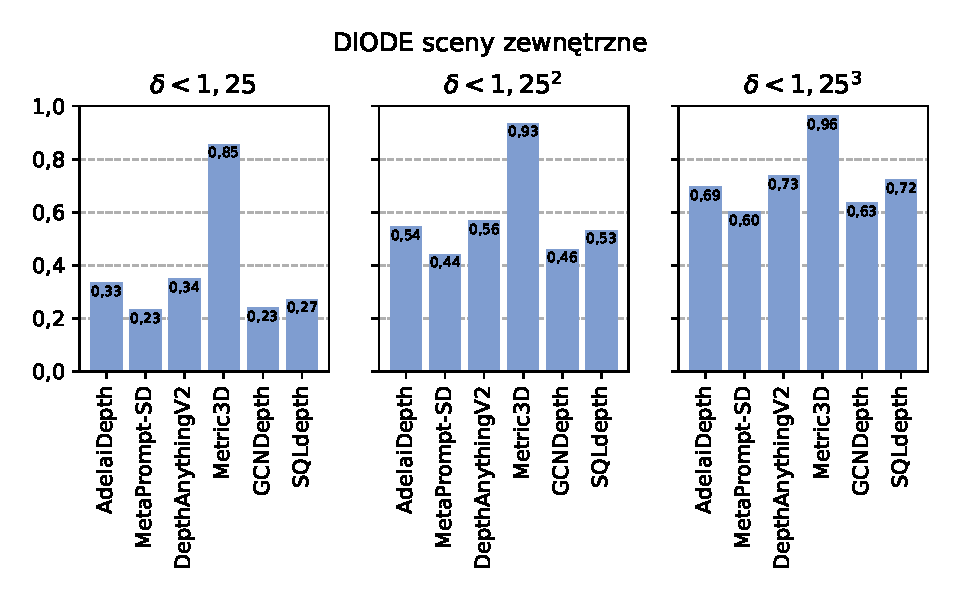
\includegraphics{plots/delta/0}
    \caption{Wyniki dokładności progowej na zbiorze DIODE na części ze scenami zewnętrznymi.}
    \label{fig:delta_0}
\end{figure}
\begin{figure}[H]
    \centering
    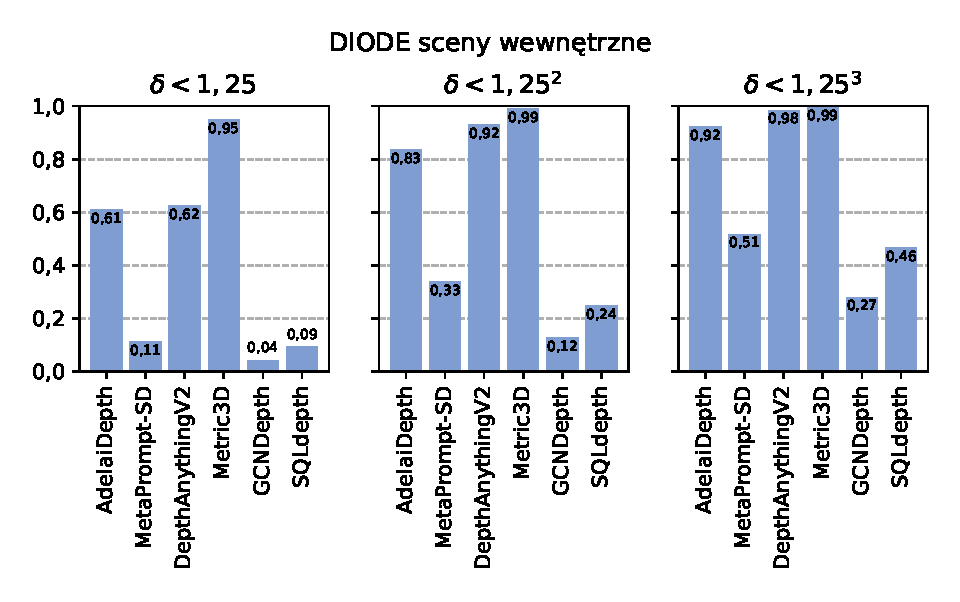
\includegraphics{plots/delta/1}
    \caption{Wyniki dokładności progowej na zbiorze DIODE na części ze scenami wewnętrznymi.}
    \label{fig:delta_1}
\end{figure}
\begin{figure}[H]
    \centering
    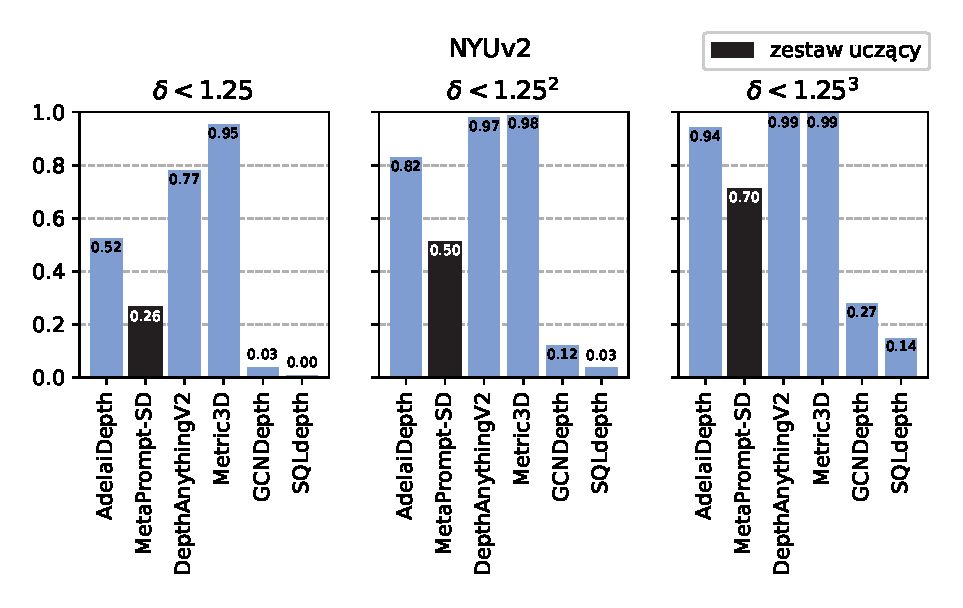
\includegraphics{plots/delta/2}
    \caption{Wyniki dokładności progowej na zbiorze NYUv2.}
    \label{fig:delta_2}
\end{figure}
\begin{figure}[H]
    \centering
    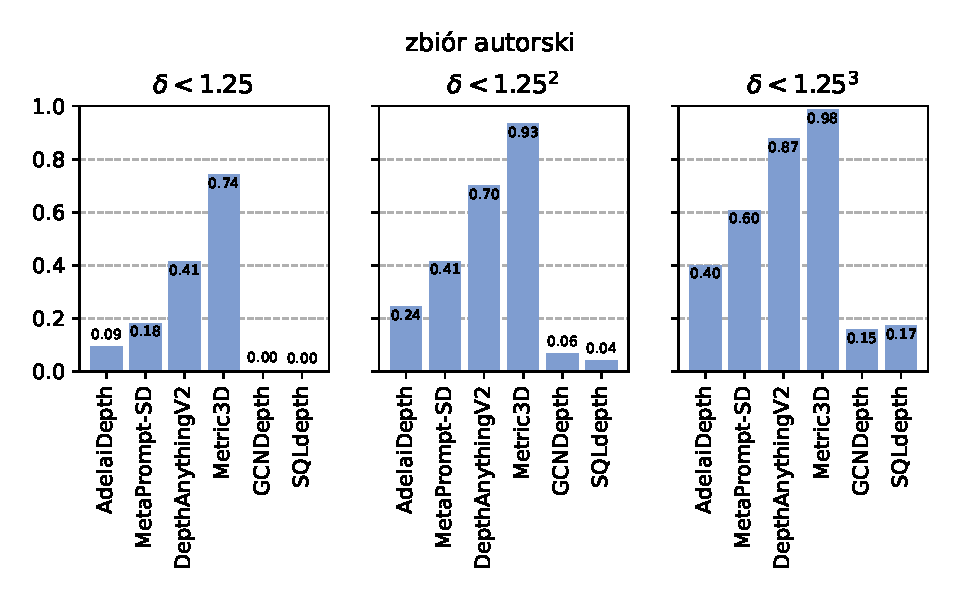
\includegraphics{plots/delta/3}
    \caption{Wyniki dokładności progowej na zbiorze autorskim.}
    \label{fig:delta_3}
\end{figure}
\begin{figure}[H]
    \centering
    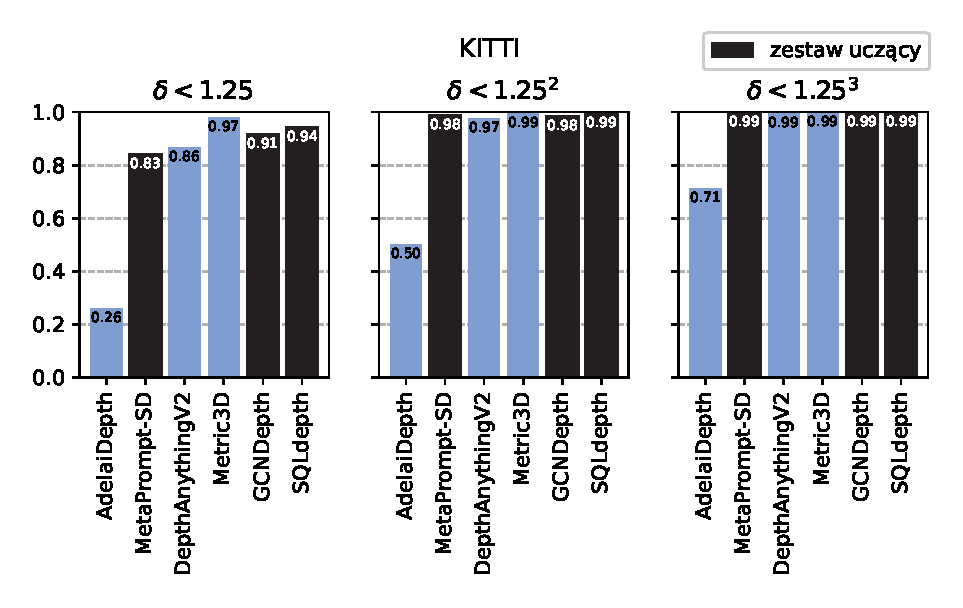
\includegraphics{plots/delta/4}
    \caption{Wyniki dokładności progowej na zbiorze KITTI.}
    \label{fig:delta_4}
\end{figure}
\begin{figure}[H]
    \centering
    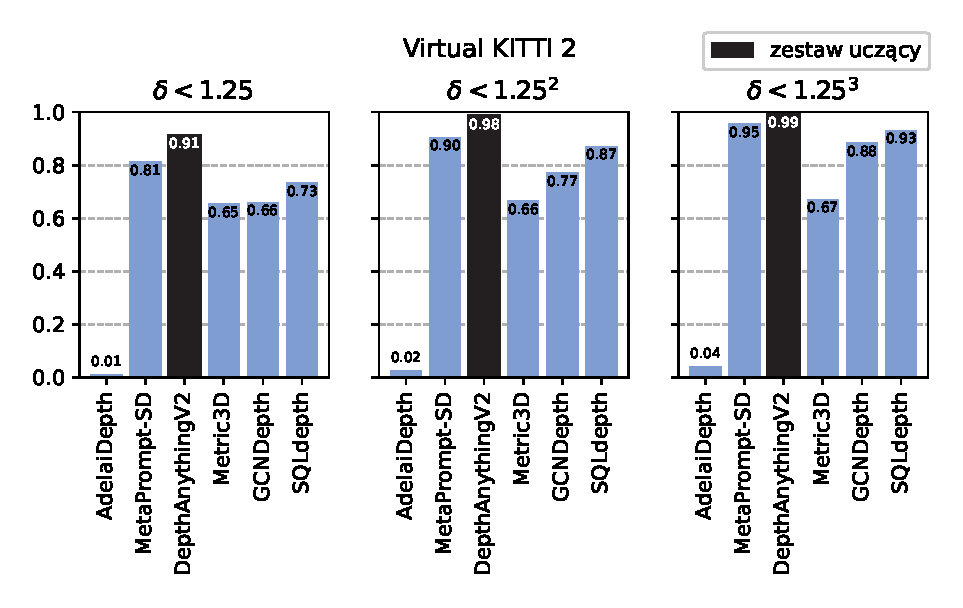
\includegraphics{plots/delta/5}
    \caption{Wyniki dokładności progowej na zbiorze Virtual KITTI 2.}
    \label{fig:delta_5}
\end{figure}
\begin{figure}[H]
    \centering
    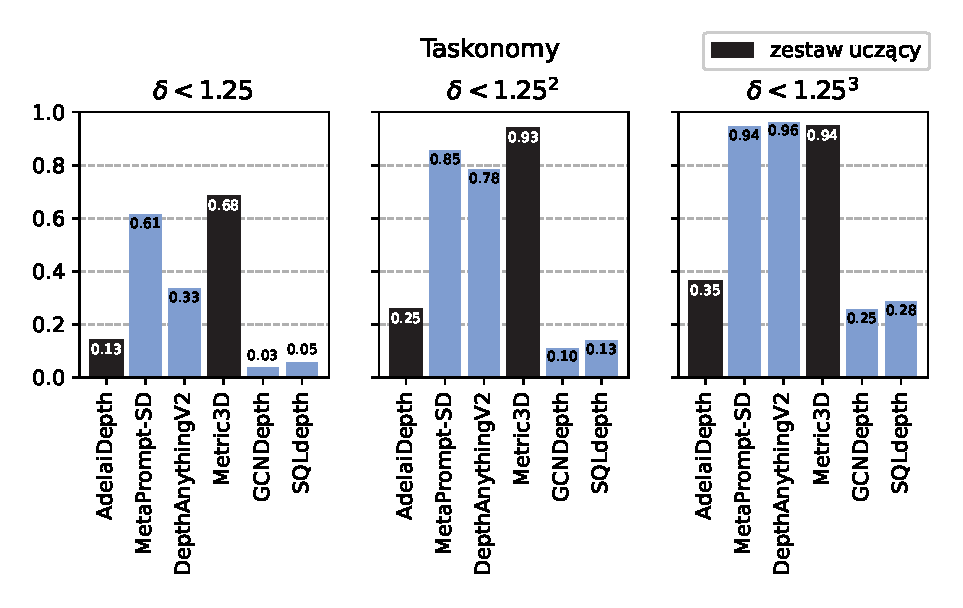
\includegraphics{plots/delta/6}
    \caption{Wyniki dokładności progowej na zbiorze Taskonomy.}
    \label{fig:delta_6}
\end{figure}

\subsection{Średni błąd bezwzględny}
Sekcja ta zawiera wyniki osiągnięte przez analizowane algorytmy w dziedzinie średniego bezwzględnego błedu estymacji \ref{eq:2}. Jest to metryka oznaczająca średnią bezwzlęgną różnicę procentową między wartościami, które są dopasowane przez algorytm, a wartościami danych rzeczywistych. Metryka ta uznawana jest za najbardziej uniwersalną, z tego powodu najczęściej występuje w publikacjach naukowych dotyczących omawianych algorytmów.

\section{Czas realizacji pojedynczej estymacji}

\section{Wymagania systemowe}
